\documentclass{article}
\usepackage{tikz}
\usetikzlibrary {shapes.geometric}
\usepackage{listings}
\title{Drawing Tree with Tikz Package}
\author{Sumaiya Tabassum}
\begin{document}
	\maketitle
	\tableofcontents
	\clearpage
	\lstset{
 language=[LaTeX]TeX,           % Set LaTeX language
 basicstyle=\ttfamily\footnotesize,
    keywordstyle=\color{blue},
    stringstyle=\color{red},
    commentstyle=\color{green!60!black},
    numbers=left,
    numberstyle=\tiny\color{gray},
    stepnumber=1,
    numbersep=10pt,
    frame=single,
    showstringspaces=false,
    breaklines=true,
    tabsize=2      
}
	\section{Introduction to the Child Operation:}
		\subsection{Basic Tree(Downward):}
		\begin{lstlisting}
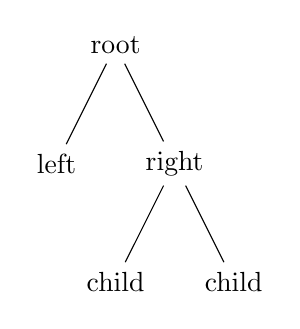
\begin{tikzpicture}
	\node {root}
		child {node{left}}
		child {node {right}
			child {node {child}}
			child {node{child}}
		};
\end{tikzpicture}
		\end{lstlisting}
		
		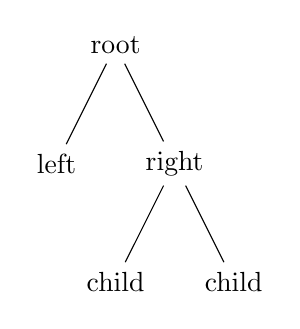
\begin{tikzpicture}
			\node {root}
				child {node{left}}
				child {node {right}
					child {node {child}}
					child {node{child}}
			};
		\end{tikzpicture}
		
		\subsection{Basic Tree(Upward):}
		\begin{lstlisting}
		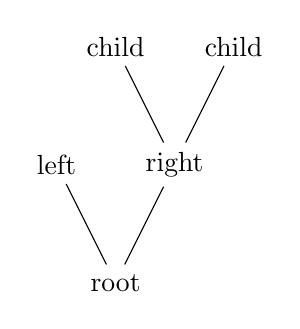
\begin{tikzpicture}
  			\node {root} [grow'=up]
    				child {node {left}}
    				child {node {right}
      				child {node {child}}
      				child {node {child}}
    			};
		\end{tikzpicture}
		
		\end{lstlisting}
		
		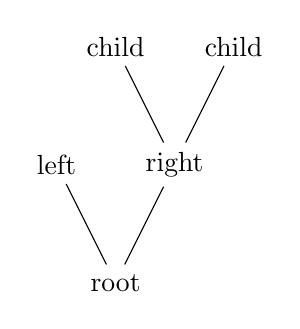
\begin{tikzpicture}
  			\node {root} [grow'=up]
    				child {node {left}}
    				child {node {right}
      				child {node {child}}
      				child {node {child}}
    			};
		\end{tikzpicture}
\pagebreak
		\subsection{Using foreach and specified distance:}

\begin{lstlisting}
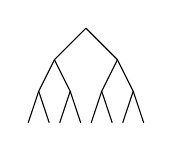
\begin{tikzpicture}[level distance = 4mm, level/.style={sibling distance=8mm/#1}]
	\coordinate
		child foreach \x in {0,1}
			{child foreach \y in {0,1}
				{child foreach \z in {0,1}}};
\end{tikzpicture}
		\end{lstlisting}		
		
		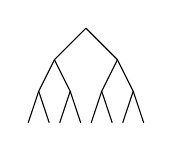
\begin{tikzpicture}[level distance = 4mm, level/.style={sibling distance=8mm/#1}]
			\coordinate
				child foreach \x in {0,1}
					{child foreach \y in {0,1}
						{child foreach \z in {0,1}}};
		\end{tikzpicture}
		
%----------------------------------------------------------------
	\section{Child Paths and Child Nodes}
		\subsection{Different Node Shapes:}
\begin{lstlisting}
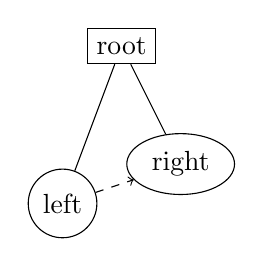
\begin{tikzpicture}[sibling distance = 15mm]
	\node[rectangle,draw] {root}
		child {node[circle,draw, yshift=-5mm](left node) {left}}
		child {node[ellipse,draw] (right node) {right}};
	\draw[dashed,->] (left node) -- (right node);
\end{tikzpicture}
\end{lstlisting}
		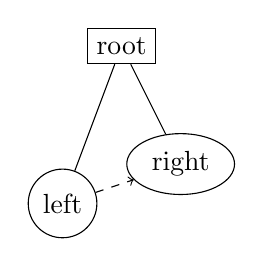
\begin{tikzpicture}[sibling distance = 15mm]
			\node[rectangle,draw] {root}
				child {node[circle,draw, yshift=-5mm](left node) {left}}
				child {node[ellipse,draw] (right node) {right}};
			 \draw[dashed,->] (left node) -- (right node);
		\end{tikzpicture}
		
		\subsection{Dot Child:}
\begin{lstlisting}
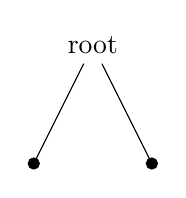
\begin{tikzpicture}
  	\node {root}
  		child {[fill] circle(2pt)}
  		child {[fill] circle(2pt)};
\end{tikzpicture}
\end{lstlisting}
		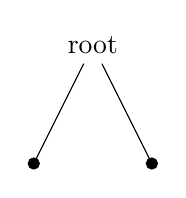
\begin{tikzpicture}
  			\node {root}
  				child {[fill] circle(2pt)}
  				child {[fill] circle(2pt)};
		\end{tikzpicture}
		
%----------------------------------------------------------------
	\section{Naming Child Nodes:}
	
\begin{lstlisting}
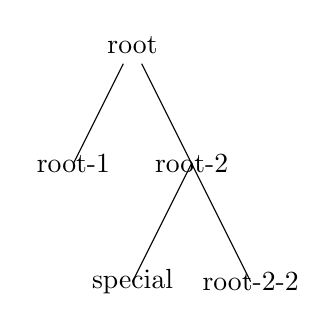
\begin{tikzpicture}
	\node(root){root}
		child
		child{
			child{coordinate(special)}
			child
		};
			
	\node at (root-1){root-1};
	\node at (root-2) {root-2};
  	\node at (special) {special};
  	\node at (root-2-2) {root-2-2};
\end{tikzpicture}
\end{lstlisting}	

	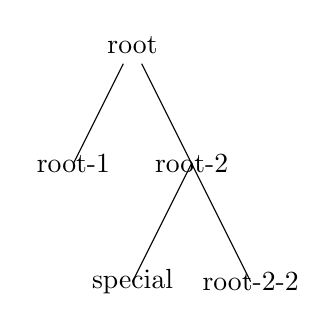
\begin{tikzpicture}
		\node(root){root}
			child
			child{
				child{coordinate(special)}
				child
			};
			
		\node at (root-1){root-1};
		\node at (root-2) {root-2};
  		\node at (special) {special};
  		\node at (root-2-2) {root-2-2};
	\end{tikzpicture}
%----------------------------------------------------------------
	\section{Specifying Options for Trees and Children:}	
	\begin{lstlisting}
\begin{tikzpicture}
  \scoped
    [...]              % Options apply to the whole tree
    \node[...] {root}  % Options apply to the root node only
       [...]           % Options apply to all children
       child[...]      % Options apply to this child and all its children
       {
         node[...] {}  % Options apply to the child node only
         ...
       }
       child[...]      % Options apply to this child and all its children
    ;
\end{tikzpicture}
\end{lstlisting}


\pagebreak
	\subsection{Branch colors:}

\begin{lstlisting}
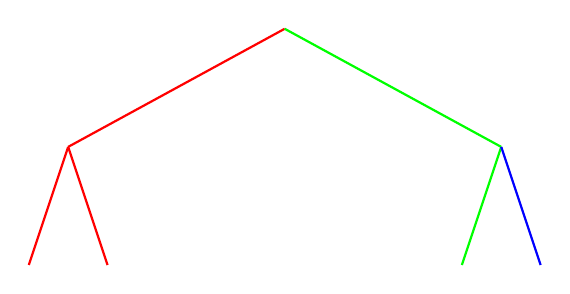
\begin{tikzpicture}[thick,level 1/.style={sibling distance=55mm}, level 2/.style={sibling distance=10mm}]
	%\node {}
	\coordinate
	child[red] {child child}
	child[green]{child child[blue]};
\end{tikzpicture}
\end{lstlisting}		

	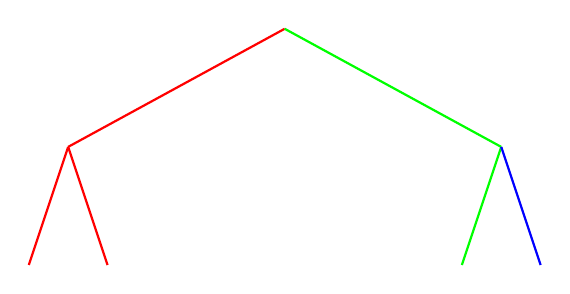
\begin{tikzpicture}[thick,level 1/.style={sibling distance=55mm}, level 2/.style={sibling distance=10mm}]
	%\node {}
	\coordinate
	child[red] {child child}
	child[green]{child child[blue]};
	\end{tikzpicture}
	
	\subsection{Node Colors:}
	
\begin{lstlisting}
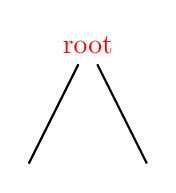
\begin{tikzpicture}[thick]
  	\node [red] {root}
    		child
   		child;
\end{tikzpicture}
\end{lstlisting}	

	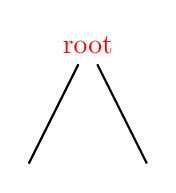
\begin{tikzpicture}[thick]
  		\node [red] {root}
    			child
   			child;
		\end{tikzpicture}
		
	\subsection{Node and Edge Colors:}

\begin{lstlisting}
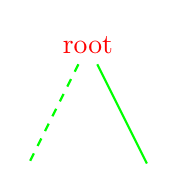
\begin{tikzpicture}[thick]
  	\node [red] {root}
    	[green] % option applies to all children
    	child[dashed]
    	child;
\end{tikzpicture}
\end{lstlisting}		

	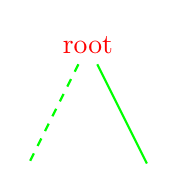
\begin{tikzpicture}[thick]
  		\node [red] {root}
    		[green] % option applies to all children
    		child[dashed]
    		child;
	\end{tikzpicture}
	
%----------------------------------------------------------------
	\section{Default Growth Function:}
	
		\subsection{Distances:}

\begin{lstlisting}
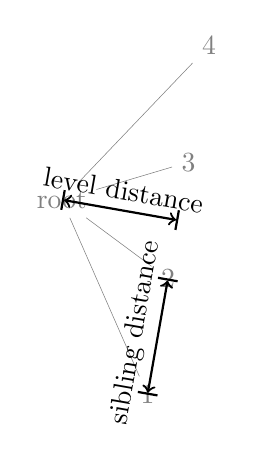
\begin{tikzpicture}[sibling distance=15mm, level distance=15mm]
  	\path [help lines]
    	node (root) {root}
    	[grow=-10]
   		child {node {1}}
    		child {node {2}}
    		child {node {3}}
    		child {node {4}};

  	\draw[|<->|,thick] (root-1.center)
    		-- node[above,sloped] {sibling distance} (root-2.center);

 	\draw[|<->|,thick] (root.center)
    		-- node[above,sloped] {level distance} +(-10:\tikzleveldistance);
\end{tikzpicture}
\end{lstlisting}	

		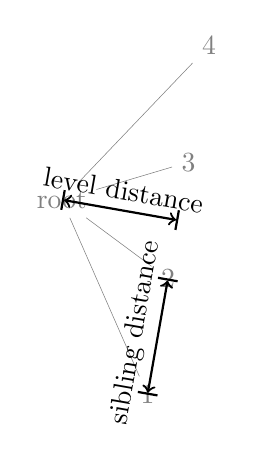
\begin{tikzpicture}[sibling distance=15mm, level distance=15mm]
  			\path [help lines]
    			node (root) {root}
    			[grow=-10]
   				child {node {1}}
    				child {node {2}}
    				child {node {3}}
    				child {node {4}};

  			\draw[|<->|,thick] (root-1.center)
    				-- node[above,sloped] {sibling distance} (root-2.center);

 			 \draw[|<->|,thick] (root.center)
    				-- node[above,sloped] {level distance} +(-10:\tikzleveldistance);
\end{tikzpicture}

\pagebreak

		\subsection{Growth Values:}
		
\begin{lstlisting}
tikz \node {root} [grow=right] child child;
\tikz \node {root} [grow=south west] child child;
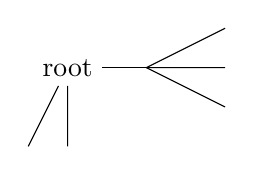
\begin{tikzpicture}[level distance=10mm,sibling distance=5mm]
  \node {root}
    [grow=down]
    child
    child
    child[grow=right] {
      child child child
    };
\end{tikzpicture}
\end{lstlisting}	

		\tikz \node {root} [grow=right] child child;
		\tikz \node {root} [grow=south west] child child;
		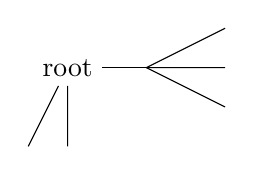
\begin{tikzpicture}[level distance=10mm,sibling distance=5mm]
  \node {root}
    [grow=down]
    child
    child
    child[grow=right] {
      child child child
    };
\end{tikzpicture}

%----------------------------------------------------------------
	\section{Missing Children:}
	
\begin{lstlisting}
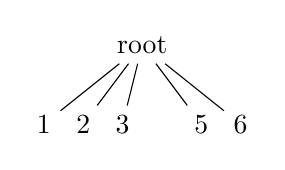
\begin{tikzpicture}[level distance=10mm,sibling distance=5mm]
  \node {root} [grow=down]
    	child          { node {1} }
    	child          { node {2} }
    	child          { node {3} }
    	child[missing] { node {4} }
    	child          { node {5} }
    	child          { node {6} };
\end{tikzpicture}
\end{lstlisting}		
	
	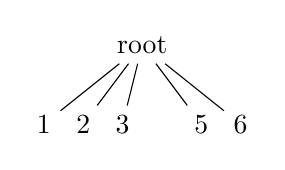
\begin{tikzpicture}[level distance=10mm,sibling distance=5mm]
  		\node {root} [grow=down]
    			child          { node {1} }
    			child          { node {2} }
    			child          { node {3} }
    			child[missing] { node {4} }
    			child          { node {5} }
    			child          { node {6} };
\end{tikzpicture}
\pagebreak
%----------------------------------------------------------------
	\section{Edges From the Parent Node:}
		\subsection{Straight Edge Variations:}
		
\begin{lstlisting}
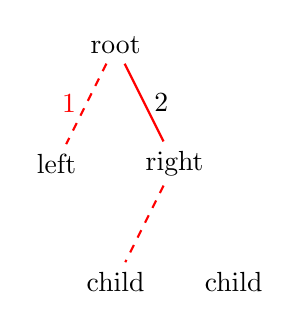
\begin{tikzpicture}[edge from parent/.style={draw,red,thick}]
	\node {root}
		child[dashed] { node {left} edge from parent[dashed] node[left]{1}}
		child {node {right} 
      		child[dashed] {node {child}}
      		child {node {child} edge from parent[draw=none]}
    		edge from parent node[black,right]{2}
    				};
\end{tikzpicture}
\end{lstlisting}		
	
		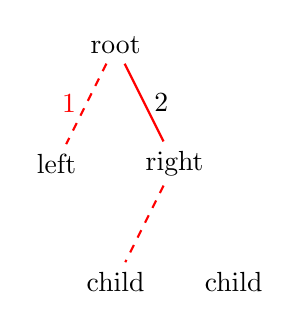
\begin{tikzpicture}[edge from parent/.style={draw,red,thick}]
			\node {root}
				child[dashed] { node {left} edge from parent[dashed] node[left]{1}}
				child {node {right} 
      				child[dashed] {node {child}}
      				child {node {child} edge from parent[draw=none]}
    				edge from parent node[black,right]{2}
    				};
		\end{tikzpicture}
		
		\subsection{Curved Edge:}

\begin{lstlisting}
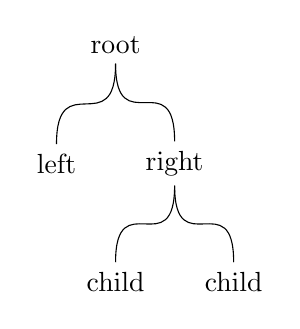
\begin{tikzpicture}[level distance=15mm, sibling distance=15mm,
  edge from parent path=
{(\tikzparentnode.south) .. controls +(0,-1) and +(0,1)
                           .. (\tikzchildnode.north)}]
  \node {root}
    child {node {left}}
    child {node {right}
      child {node {child}}
      child {node {child}}
    };
\end{tikzpicture}
\end{lstlisting}			

			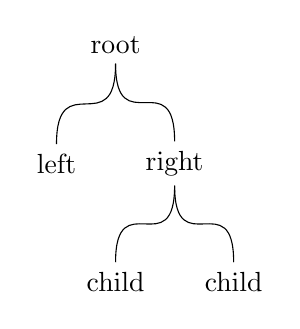
\begin{tikzpicture}[level distance=15mm, sibling distance=15mm,
  edge from parent path=
{(\tikzparentnode.south) .. controls +(0,-1) and +(0,1)
                           .. (\tikzchildnode.north)}]
  \node {root}
    child {node {left}}
    child {node {right}
      child {node {child}}
      child {node {child}}
    };
\end{tikzpicture}
%----------------------------------------------------------------
	\section{Practice}
	\subsection{Practice 01:}
	
\begin{lstlisting}
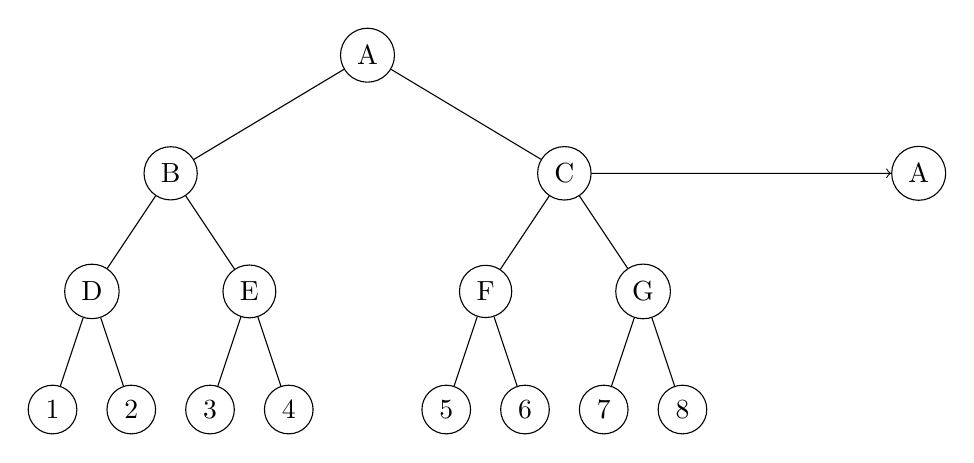
\begin{tikzpicture}
	[every node/.style={circle,draw},
	level 1/.style={sibling distance=50mm},
	level 2/.style={sibling distance=20mm},
	level 3/.style={sibling distance=10mm}]
		\node{A}
			child {node {B}
				child{node{D}
					child{node{1}}
					child{node{2}}
				}
				child{node {E}
					child{node{3}}
					child{node{4}}				
				}
			}
			child {node(1) {C}
				child{node{F}
					child{node{5}}
					child{node{6}}				
				}
				child{node{G}
					child{node{7}}
					child{node{8}}				
				}
			};
			\node(2) at (7,-1.5){A};
			\draw[->](1) to (2);
	\end{tikzpicture}
\end{lstlisting}	

	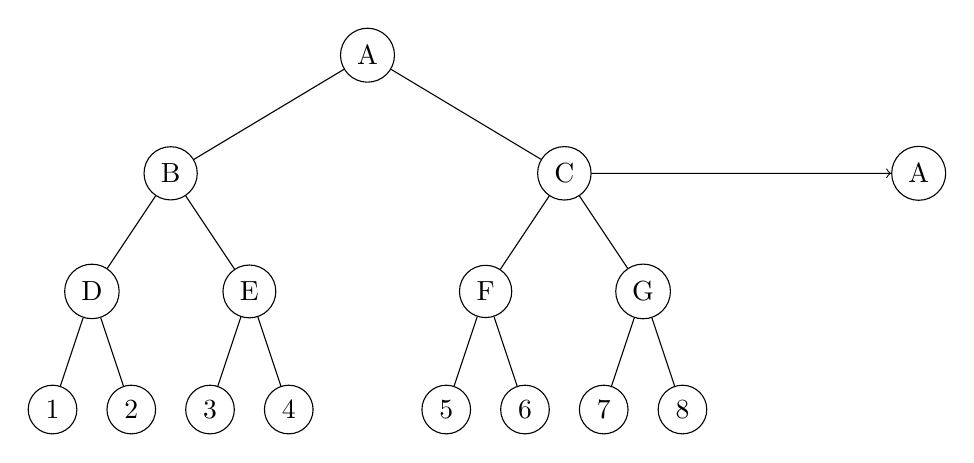
\begin{tikzpicture}
	[every node/.style={circle,draw},
	level 1/.style={sibling distance=50mm},
	level 2/.style={sibling distance=20mm},
	level 3/.style={sibling distance=10mm}]
		\node{A}
			child {node {B}
				child{node{D}
					child{node{1}}
					child{node{2}}
				}
				child{node {E}
					child{node{3}}
					child{node{4}}				
				}
			}
			child {node(1) {C}
				child{node{F}
					child{node{5}}
					child{node{6}}				
				}
				child{node{G}
					child{node{7}}
					child{node{8}}				
				}
			};
			\node(2) at (7,-1.5){A};
			\draw[->](1) to (2);
	\end{tikzpicture}
	
\pagebreak	
	\subsection{Practice 02:}
	
\begin{lstlisting}
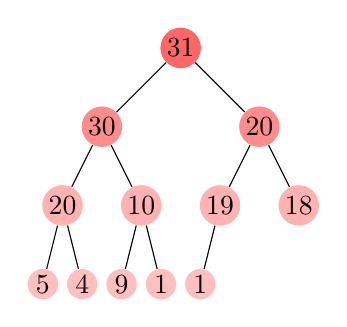
\begin{tikzpicture}
  	[level distance=10mm,
   	every node/.style={fill=red!60,circle,inner sep=1pt},
  	level 1/.style={sibling distance=20mm,nodes={fill=red!45}},
   	level 2/.style={sibling distance=10mm,nodes={fill=red!30}},
	level 3/.style={sibling distance=5mm,nodes={fill=red!25}}]
  	\node {31}
     	child {node {30}
       		child {node {20}
        	  		child {node {5}}
         		child {node {4}}
       		}
       		child {node {10}
         		child {node {9}}
         		child {node {1}}
       		}
    		}
     	child {node {20}
       		child {node {19}
         		child {node {1}}
         	child[missing]
       		}
       		child {node {18}}
     	};
\end{tikzpicture}
\end{lstlisting}	

	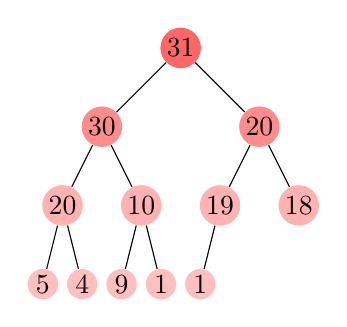
\begin{tikzpicture}
  		[level distance=10mm,
   		 every node/.style={fill=red!60,circle,inner sep=1pt},
  		 level 1/.style={sibling distance=20mm,nodes={fill=red!45}},
   		 level 2/.style={sibling distance=10mm,nodes={fill=red!30}},
		 level 3/.style={sibling distance=5mm,nodes={fill=red!25}}]
  		\node {31}
     		child {node {30}
       			child {node {20}
        	  			child {node {5}}
         			child {node {4}}
       			}
       			child {node {10}
         			child {node {9}}
         			child {node {1}}
       			}
    			}
     		child {node {20}
       			child {node {19}
         			child {node {1}}
         		child[missing]
       			}
       			child {node {18}}
     		};
\end{tikzpicture}
		
\end{document}
